\chapter{Konzeption der Megamap-Anwendung}
\label{chap:concept}
In diesem Kapitel wird das Konzept der Megamap erläutert.
Zunächst wird der Begriff der Kartenexploration definiert.
Als Inspiration für das Konzept werden danach die Elemente aus existierenden Kartenanwendungen analysiert, welche die Exploration von Umgebungen ermöglichen.
Diese Elemente werden kategorisiert, zusammengefasst und schließlich als Grundlage für das Megamap-Konzept verwendet.

\section{Definition Kartenexploration}
\label{sec:definition_exploration}
% Hier die Guidelines einarbeiten
Bereits \textcite{Reichenbacher2001} beschreibt Konzepte zur mobilen Nutzung von digitalen Kartensystemen.
Er gibt eine Übersicht verschiedener \emph{User Tasks}, die in mobilen Umgebungen ausgeführt werden können (siehe \autoref{tab:gis_user_tasks}).
Einer dieser User Tasks ist die \textbf{Navigation}, welche in digitalen Kartensystemen durch Wegbeschreibungen umgesetzt wird.
Die Nutzer bekommen Pfade zwischen zwei Punkten angezeigt, die den schnellsten oder den kürzesten Weg zum Ziel anschaulich machen.
Zusätzlich können wegweisende Textinformationen die Navigation erleichtern.
\begin{table}[htb]
    \centering
    \caption{Geoinformationsaufgaben in einer mobilen Umgebung. \quelle{\cite{Reichenbacher2001}}}
    \label{tab:gis_user_tasks}
    \begin{tabular}{@{}lll@{}}%\toprule
        \tableheadcolor \textsf{\textbf{Tasks}} & \textsf{\textbf{Subtasks}} & \textsf{\textbf{Examples}}\\% \midrule
        \rowcolorodd & Own position & xy coordinates, place name \\
        \rowcolorodd & Objects & Attributes of an object\\
        \rowcolorodd \multirow{-3}{*}{Locators} & Other persons position & Who is this?\\% \midrule
        \rowcoloreven & Objects & Next object with certain attributes\\
        \rowcoloreven \multirow{-2}{*}{Proximity} & Persons & Known people in the area?\\% \midrule
        \rowcolorodd Navigation & Routing & Way descriptions\\% \midrule
        \rowcoloreven Events & What happens at a place & Obstacles (e.g. traffic jam)?\\% \bottomrule
    \end{tabular}
    \vspace{0.5em}
\end{table}

Neben der Navigation nennt \citeauthor{Reichenbacher2001} drei weitere Kategorien von User Tasks:
\begin{itemize}
    \item \textbf{Lokalisierungs-Tasks (\emph{Locators})} sind Anwendungsfälle, bei denen die Nutzer Positionen von spezifischen Orten abfragen und dazu Informationen über die Attribute des Orts erhalten.
    
    \item \textbf{Nähe-Tasks (\emph{Proximity})} sind Anwendungsfälle, bei denen die Nutzer anhand vorgegebener Attribute nach zutreffenden Orten suchen.
    So kann z.\,B. die Umgebung nach den nächstgelegenen Geschäften oder Freizeitbeschäftigungen durchsucht werden.
    
    \item Bei \textbf{Events} geht es um die Abfrage von Informationen der Umgebung mit zeitlichem Bezug.
    Beispielsweise fällt die Suche nach geöffneten Geschäften oder die Anzeige von Echtzeitverkehrsinformationen in diese Kategorie.
\end{itemize}

Die abgefragten Informationen sind abhängig von \emph{mindestens} einem Kontext, zum Beispiel der aktuellen Position der Nutzers.
Es können aber auch mehrere Kontexte gleichzeitig mit einbezogen werden (Beispiel: \enquote{Alle \emph{Geschäfte} in \emph{der Nähe}, die \emph{zurzeit} geöffnet sind} $\rightarrow$ \mbox{Zweck-}, Positions- und Zeitkontext).
Dies steht im Kontrast zur Navigation, für welche immer ein Endpunkt im Kontext zu \emph{mindestens} einem Startpunkt stehen muss (weitere Kontexte wären z.\,B. Zwischenstopps, das genutzte Fortbewegungsmittel oder das aktuelle Verkehrsaufkommen).
Da die Nutzer eine Umgebung durch Abfragen der Umgebungsinformationen \enquote{entdecken}, wird \textbf{Kartenexploration} als Oberbegriff für die oben beschriebenen Lokalisierungs-, Nähe- und Event-Tasks betrachtet.

\section{Explorationselemente in existierenden Kartenanwendungen}
\label{sec:exploration_elements}
Kartenanwendungen setzen unterschiedliche Elemente ein, um die digitale Kartenexploration zu ermöglichen.
Bevor das Konzept für die Megamap formuliert wird, werden die Darstellungselemente und Interaktionsmöglichkeiten zur Kartenexploration in bereits existierenden Anwendungen gesammelt und kategorisiert.
Die Idee ist, diejenigen Elemente für das Megamap-Konzept zu übernehmen, die den Nutzern bereits aus den anderen Anwendungen bekannt sind.
So sollen die Nutzer die Bedienung der Megamap schneller verstehen und lernen können.
Die gesammelten Elemente und Interaktionsmöglichkeiten werden jeweils den User Tasks aus \autoref{sec:definition_exploration} zugeordnet.
Demnach ergeben sich drei Kategorien von Explorationselementen: \textbf{Lokalisierungselemente}, \textbf{Nähe-Elemente} und \textbf{Event-Elemente}.

Als Beispiele für existierende Kartenanwendungen wurden die Web-Varianten von \emph{Google~Maps}\parencite{GoogleLLC2018}, \emph{Bing Maps} \parencite{Microsoft2018b} und \emph{HERE WeGo} \parencite{HERE2018} untersucht.
Alle drei Webseiten bieten neben der Routen-Planung auch Funktionen zur Erkundung von Umgebungen an.
\autoref{tab:exploration_elements_summary} zeigt eine Übersicht der analysierten Explorationselemente.
Die einzelnen Elemente werden in den folgenden Abschnitten mit Beispielen näher erläutert.

\begin{table}[tbh]
    \small
    \centering
    \caption{Übersicht der Explorationselemente in ausgewählten Anwendungen, eingeschlossen der Megamap aus TCTD.}
    \label{tab:exploration_elements_summary}
    \begin{tabular}{@{}lcccc@{}}
        \tableheadcolor
        \textsf{\textbf{Explorationselement}} & \rotatebox[origin=c]{90}{\textsf{\textbf{\hspace{2mm}Google Maps\hspace{2mm}}}} & \rotatebox[origin=c]{90}{\textsf{\textbf{Bing Maps}}} & \rotatebox[origin=c]{90}{\textsf{\textbf{Here WeGo}}} & \rotatebox[origin=c]{90}{\textsf{\textbf{TCTD}}} \\

        \tableheadcolor
        \multicolumn{5}{@{}l@{}}{\textsc{Lokalisierung}} \\
        \rowcolorodd Positionsmarker (Nutzer) & \checkmark & \checkmark & \checkmark & \checkmark \\
        \rowcoloreven Labels (Straßen, Flüsse, \dots) & \checkmark & \checkmark & \checkmark & \checkmark \\
        \rowcolorodd Ortsmarkierungen & \checkmark & \checkmark & \checkmark &  \checkmark \\
        \rowcoloreven Klickmarkierung (Adresse, Koordinaten) & \checkmark & \checkmark & \checkmark & \checkmark \\
        \rowcolorodd Spezifische Suche (mittels Suchfeld) & \checkmark & \checkmark & \checkmark & --- \\
        \rowcoloreven Attributsübersicht & \checkmark & \checkmark & --- & \checkmark \\

        \tableheadcolor \multicolumn{5}{@{}l@{}}{\textsc{Nähe}} \\
        \rowcolorodd Ortsmarkierungen (Positionsabh.) & \checkmark & \checkmark & \checkmark & \checkmark \\
        \rowcoloreven Ortsmarkierungen (Zoomabh.) & \checkmark & \checkmark & \checkmark & \checkmark \\
        \rowcolorodd Entfernungen (außerhalb Navigation) & \checkmark & \checkmark & --- & \checkmark \\
        \rowcoloreven Offene Suche (mittels Suchfeld) & \checkmark & \checkmark & \checkmark & --- \\
        \rowcolorodd Nahbereichssuche & \checkmark & \checkmark & --- & --- \\
        \rowcoloreven Filter u. Sortierung & \checkmark & \checkmark & --- & Nur Filter \\
        \rowcolorodd Ortsnachbarschaft & \checkmark & \checkmark & Nur Transport & --- \\
        \rowcoloreven Umgebungsbilder & \checkmark & \checkmark & --- & --- \\

        \tableheadcolor \multicolumn{5}{@{}l@{}}{\textsc{Event}} \\
        \rowcolorodd Öffnungszeiten & \checkmark & \checkmark & \checkmark & --- \\
        \rowcoloreven Verkehrsinformationen & \checkmark & \checkmark & \checkmark & --- \\
        \rowcolorodd Veranstaltungen & \checkmark & --- & --- & --- \\
        \rowcoloreven Besucheraufkommen & \checkmark & --- & --- & --- \\

    \end{tabular}
\end{table}

\subsection{Lokalisierungselemente}
\label{ssec:loc-elements}
Lokalisierungselemente sind solche, die wichtige oder interessante Orte auf der Karte markieren oder Eigenschaften von spezifischen Orten preisgeben.
Die Untersuchung der Beispielanwendungen ergab sechs Arten von Lokalisierungselementen:

Der \emph{Positionsmarker} ist ein grafisches Element auf der Karte, der die aktuelle Position der Nutzer (und unter Umständen auch die Blickrichtung) repräsentiert.
Ein Beispiel findet sich in \autoref{fig:gm_positionsmarker}.
Die Standortdienste des jeweiligen Endgeräts werden benutzt, um den Marker auf der Karte zu platzieren.
Der Positionsmarker erlaubt es, die eigene Position in der Umgebung zu bestimmen.

\emph{Labels} sind Textelemente, welche die Namen von Straßen, Flüssen, Gebäuden etc. auf der Karte zeigen (siehe \autoref{fig:hwg_labels}).
Nutzer können Kartenlabels mit Schildern und Wegweisern in der Umgebung abgleichen, was die Orientierung erleichtert.
Da Orte auf der Karte und in der Umgebung explizit benannt sind, können die Namen für eindeutige Wegbeschreibungen eingesetzt werden.
\begin{figure}[h]
    \centering
    \begin{minipage}[t]{.485\textwidth}
        \centering
        \vspace{0pt}
        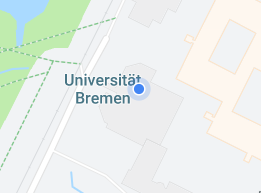
\includegraphics[width=\linewidth, height=4.5cm]{figures/map-app_examples/gm_positionsmarker}
        \captionof{figure}{Beispiel eines Positionsmarkers in Google Maps.}
        \label{fig:gm_positionsmarker}
        \vfill
    \end{minipage}
    \hfill
    \begin{minipage}[t]{.485\textwidth}
        \centering
        \vspace{0pt}
        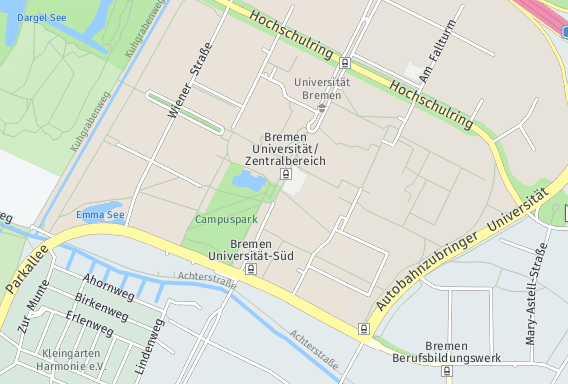
\includegraphics[width=\linewidth, height=4.5cm]{figures/map-app_examples/hwg_labels}
        \captionof{figure}{Beispiel von Labels in HERE WeGo.}
        \label{fig:hwg_labels}
    \end{minipage}
\end{figure}

\emph{Ortsmarkierungen} sind grafische Elemente, welche die Positionen von gewissen Gebäuden oder anderen interessanten Punkten (\emph{Points-of-Interest}, POI) auf Karten markieren.
Es gibt sowohl statische Ortsmarkierungen, die zusammen mit den Labels auf der Karte fest verankert sind, wie auch dynamische Ortsmarkierungen, die je nach Kontext des Nutzers ein- bzw. ausgeblendet werden.
Die dynamischen Ortsmarkierungen werden durch \enquote{Stecknadeln} repräsentiert.
Sie sind mit Icons versehen, die die Art des POI anzeigen.
Beispiele finden sich in \autoref{fig:bm_gebaeudemarkierungen}.

Eine \emph{Klickmarkierung} kann in den Kartenanwendungen durch Klicken auf den Kartenbereich erzeugt werden.
Die Markierung wird grafisch als Stecknadel oder ein vergleichbares Symbol dargestellt (siehe \autoref{fig:gm_klickmarkierung}).
Über eine solche Markierung können Nutzer auf die Adresse und/oder die Koordinaten am angeklickten Ort zugreifen.
\begin{figure}[t]
    \centering
    \begin{minipage}[t]{.485\textwidth}
        \centering
        \vspace{0pt}
        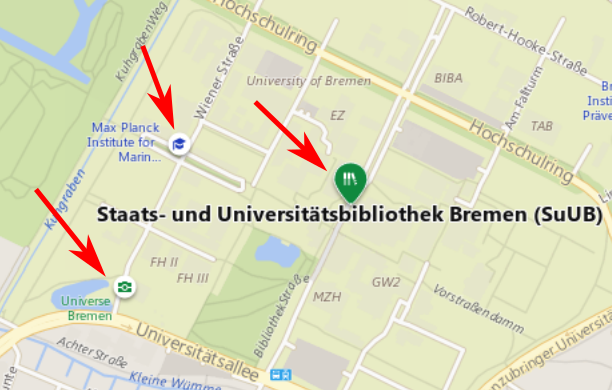
\includegraphics[width=\linewidth, height=4.5cm]{figures/map-app_examples/bm_gebaeudemarkierungen_arrows}
        \captionof{figure}{Beispiel von Ortsmarkierungen in Bing Maps (hervorgehoben durch \textcolor{red}{rote} Pfeile). %
        Ausgewählte Orte werden durch Stecknadeln stärker betont.}
        \label{fig:bm_gebaeudemarkierungen}
        \vfill
    \end{minipage}
    \hfill
    \begin{minipage}[t]{.485\textwidth}
        \centering
        \vspace{0pt}
        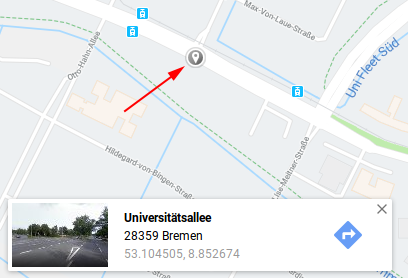
\includegraphics[width=\linewidth, height=4.5cm]{figures/map-app_examples/gm_klickmarkierung}
        \captionof{figure}{Beispiel der Klickmarkierung in Google Maps (hervorgehoben durch \textcolor{red}{roten} Pfeil). %
        Unterhalb der Markierung werden die Adresse und Koordinaten gezeigt.}
        \label{fig:gm_klickmarkierung}
    \end{minipage}
\end{figure}

Die \emph{spezifische Suche} ist eine Lokalisierungs-Interaktion, die durch ein Suchfeld ausgelöst wird.
Als \emph{spezifische} Suche (im Gegensatz zur \emph{offenen} Suche) wird in dieser Arbeit die Suche nach einer bekannten Adresse oder einem eindeutig benannten Ort verstanden (beispielsweise \enquote{Bremer Rathaus} oder \enquote{Bibliothekstraße 1}).
Wird eine solche Suche durchgeführt, platziert die Anwendung eine grafische Markierung auf dem Zielobjekt.
Den Nutzern bleibt somit eine manuelle Suche nach dem Zielort auf der Karte erspart.

Das letzte Lokalisierungselement ist die \emph{Attributsansicht}.
Über diese Ansicht werden den Nutzern Informationen über einen Ort aufgelistet.
Die Informationen umfassen neben der Adresse und Anschrift unter anderem auch Kontaktdaten (Webseiten, Telefonnummern), Öffnungszeiten, Bilder, Bewertungen usw.
Speziell für Gebäude werden hier auch Ausstattungen gelistet.
Die Anzeige solcher Informationen ermöglicht es, die Kartenanwendungen für andere Anwendungsfälle als die reine Navigation zu nutzen.
Beispielsweise können Nutzer mit der Kartenanwendung ihre Unterkunft während einer Reise planen und werden dann zur Buchung auf die jeweilige Seite des Hotels weitergeleitet.

\subsection{Nähe-Elemente}
\label{ssec:prox-elements}
Nähe-Elemente sind Explorationselemente, die im Bezug zur Position der Nutzer stehen.
Sie werden miteinander kombiniert, um einen Überblick der Umgebung als Ganzes zu geben.
Vor allem bei der offenen Suche nach unspezifischen Orten (z.\,B. \enquote{Restaurants in der Nähe}) kommen die Nähe-Elemente zum Einsatz, indem mehrere Alternativen als Zielorte angeboten werden.
Bei der Untersuchung der Beispielanwendungen ergaben sich acht Arten von Nähe-Elementen:

\emph{Positionsabhängige Ortsmarkierungen} werden nur in der näheren Umgebung des Nutzers eingeblendet.
So können sich Nutzer auf nahegelegene Alternativen konzentrieren und die weiter entfernten Ziele ausblenden.
Erweitert wird dies durch die \emph{zoomabhängigen Ortsmarkierungen}, deren Sichtbarkeit vom Zoom der Karte abhängt.
Die Anbieter der Kartenanwendung können damit zum Beispiel beliebte, häufig frequentierte Ziele hervorheben, während wenig besuchte Ziele ausgeblendet werden.

\emph{Entfernungen} können als Nähe-Elemente außerhalb der reinen Navigation eingesetzt werden, um konkrete Entfernungsverhältnisse in der Umgebung anzuzeigen.
Entfernungen werden zum Beispiel zusammen mit anderen Ortsinformationen angezeigt, oder Nutzer benutzen ein virtuelles Maßband zum Abmessen auf der digitalen Karte.
Nutzer können dadurch Reisezeiten abschätzen und bei mehreren Zielalternativen die mit dem kürzesten Reiseweg wählen.

Die \emph{offene Suche} ist eine Nähe-Interaktion, die über ein Suchfeld ausgelöst wird.
Anders als die \emph{spezifische} Suche wird bei der offenen Suche nach Attributen von Orten gesucht (z.\,B. die Kategorien \enquote{Restaurants}, \enquote{Parks}, \enquote{Zoo}).
Den Nutzern werden alle zutreffende Zielalternativen innerhalb eines Bereichs angezeigt, sodass sie zwischen diesen auswählen können.
In den untersuchten Anwendungen werden alle möglichen Alternativen durch Ortsmarkierungen hervorgehoben.
\autoref{fig:bm_open_search} zeigt eine offene Suche nach Hotels in Bremen.
\begin{figure}[h]
	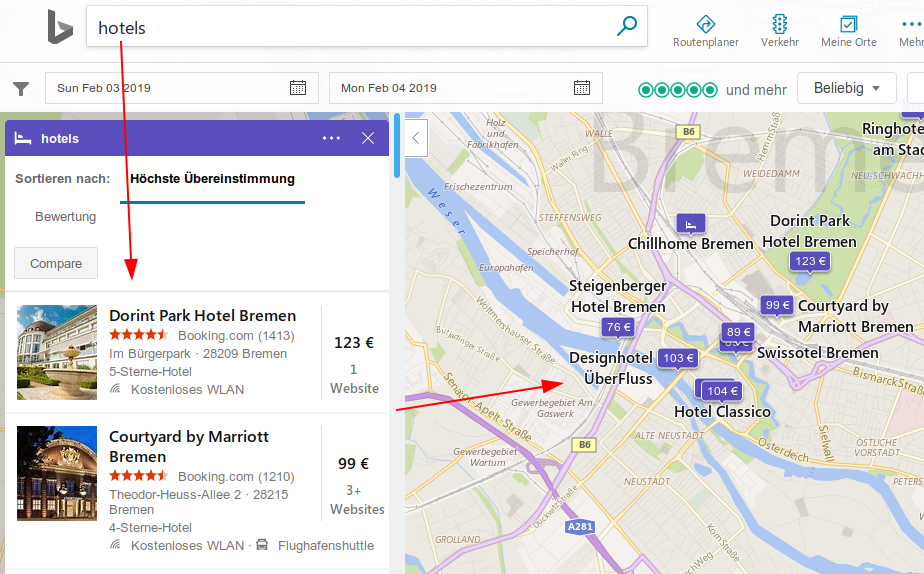
\includegraphics[width=\linewidth]{figures/map-app_examples/bm_open_search_2}
	\caption{Offene Suche nach Hotels in Bing Maps liefert mehrere Alternativen.}
	\label{fig:bm_open_search}
\end{figure}

Die \emph{Nahbereichssuche} ist eine Interaktion, mit der ein definierter Bereich der Karte unter Suchkriterien nach Orten durchsucht werden kann.
Damit ist sie eine lokal begrenzte, offene Suche.
In den Anwendungen lässt sich diese Funktion durch Öffnen des Kartenmenus mittels Rechtsklick aufrufen.
Bei der Nahbereichssuche werden nur Ortsmarkierungen angezeigt, die sich in einem gewissen Radius um den Ort des Anklickens herum befinden.
Nutzer können hiermit Umgebungen erkunden, an denen sie sich selber nicht befinden.

Über die Elemente \emph{Filter und Sortierung} können die Suchkriterien weiter eingeschränkt werden.
Beispielsweise lassen sich Restaurants nach der gewünschten Küche filtern (siehe \autoref{fig:bm_sorting}), oder Hotels nach Preisklasse.
So müssen die Nutzer nicht sämtliche verfügbare Alternativen per Hand durchgehen, um zu prüfen, ob die Alternativen ihren Vorstellungen entsprechen.
Sie können mit der Filterung und Sortierung irrelevanter Orte ausblenden und beim Suchen von Zielen Zeit sparen.
\begin{figure}[h]
    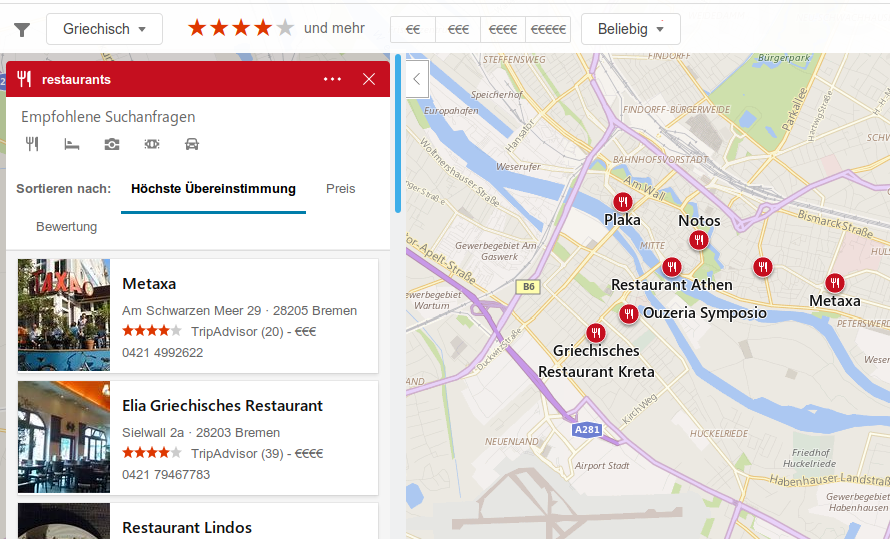
\includegraphics[width=\linewidth]{figures/map-app_examples/bm_filter_sorting}
    \caption{Anzeige und Sortierung von griechischen Restaurants mit einer 4-Sterne-Bewertung oder höher (in Bing Maps).}
    \label{fig:bm_sorting}
\end{figure}

Das Nähe-Element \emph{Ortsnachbarschaft} ist ein Element, welches in der Ansicht über die Ortsinformationen integriert ist.
Hierbei handelt es sich um eine Liste von weiteren Nutzer-relevanten Orten, die sich in der Nähe des aktuell betrachteten Orts befinden.
Auch die Information über nahegelegene Transportmöglichkeiten fällt unter diese Kategorie.

Schließlich finden sich \emph{Umgebungsbilder} in den Kartenanwendungen als Nähe-Element.
Sie zeigen Foto-Aufnahmen (gegebenenfalls als 360\textdegree-Aufnahme) der Umgebung.
Wie die Ortsmarkierungen sind die abgebildeten Orte auf einen gewissen Radius um einen Ausgangspunkt herum beschränkt, sodass nur für die Nutzer relevante Bilder zu sehen sind.
Die Einbindung der Bilder in die Anwendungen wird unterschiedlich gehandhabt.
Zum Beispiel befindet sich in Google~Maps eine Liste von Umgebungsfotos in Attributsansicht.
Wird die Liste angeklickt, öffnet sich eine Großansicht der Fotos.
Handelt es sich bei dem Bild um eine 360\textdegree-Aufnahme, kann mit der Maus die Ansicht verändert werden.

\subsection{Event-Elemente}
\label{ssec:event-elements}
Event-Elemente integrieren zeitliche Geschehnisse in die digitalen Karten.
Die Eventinformationen werden in Echtzeit aus diversen Datenquellen bezogen, um die Karte zu aktualisieren.
Bei der Untersuchung der Beispielanwendungen ergaben sich vier Arten von Event-Elementen:

Die \emph{Verkehrsinformationen} informieren Nutzer über die aktuelle Situation des Straßenverkehrs.
Verkehrsaufkommen, Baustellen, Staus und Umleitungen werden in die Karten integriert und visualisiert.
Neben der aktuellen Verkehrssituation werden auch Durchschnittswerte für die Befahrung von Straßen angezeigt, sodass die Nutzer bereits vor der Abfahrt den Verkehr in der Umgebung abschätzen können.

Die \emph{Veranstaltungsinformationen} sind in die Ortsinformationen integriert.
Hier werden die Veranstaltungen der nächsten Tage präsentiert (z.\,B. Konzerte).
Unter Umständen werden auch die Ticketverfügbarkeit und -preise angezeigt.

Für Gebäude auf der Karte werden \emph{Öffnungszeiten} angezeigt.
Dank der Integration der Öffnungszeiten müssen die Nutzer keine anderen Anwendungen oder Websites aufrufen, um zu schauen, ob das Ziel zur aktuellen Zeit erreicht werden kann.
Schließlich sind auch Informationen über das \emph{aktuelle Besucheraufkommen an Orten} als Event-Element verfügbar.
Die Nutzer können zum Beispiel einsehen, ob ein großer Andrang auf ein Geschäft besteht und so lange Wartezeiten beim Schlangestehen vermeiden.

\section{Megamap in \emph{Tom Clancy's The Division}}
In \autoref{chap:einleitung} wurde bereits erwähnt, dass die grundlegende Idee für das Konzept der Megamap aus dem Spiel Tom Clancy's The Division stammt.
Anders als die zuvor beschriebenen Kartenanwendungen implementiert die Megamap in TCTD eine dreidimensionale Karte, basierend auf einem virtuellen New York.
Die Karte wird in die Umgebung des Spielcharakters integriert, sodass dieser \enquote{in der Karte steht}.
Aus der Sicht des Spielcharakters handelt es sich also um eine AR-Karte.

Im Vergleich zu den vorigen Kartenanwendungen lassen sich sowohl Gemeinsamkeiten als auch Unterschiede bei der Umsetzung der Explorationselemente ermitteln.
Für diese Arbeit wird die Megamap aus TCTD als vierte \enquote{Kartenanwendung} nach den gleichen Kriterien wie die anderen Anwendungen betrachtet.
Dieser Abschnitt geht auf die Explorationselemente in TCTDs Megamap ein.
Eine Übersicht der gefundenen Elemente findet sich (zusammen mit denen der anderen Anwendungen) in \autoref{tab:exploration_elements_summary}.

Das Aufrufen der Megamap in TCTD geschieht in zwei Schritten (siehe \autoref{fig:tctd_overview}):
\begin{enumerate}
    \item Ein kleiner Ausschnitt der Megamap wird um den Spielcharakter herum in die virtuelle Umgebung integriert.
    Falls sich dort bereits Objekte befinden, bleiben diese weiterhin sichtbar.
    Die Megamap ist an den Überschneidungspunkten komplett transparent.
    \item Sobald sich der Kartenausschnitt durch den Spieler ändert, wird die Umgebung ausgeblendet und nur die Megamap bleibt sichtbar.
\end{enumerate}
\begin{figure}[h!]
    \centering
    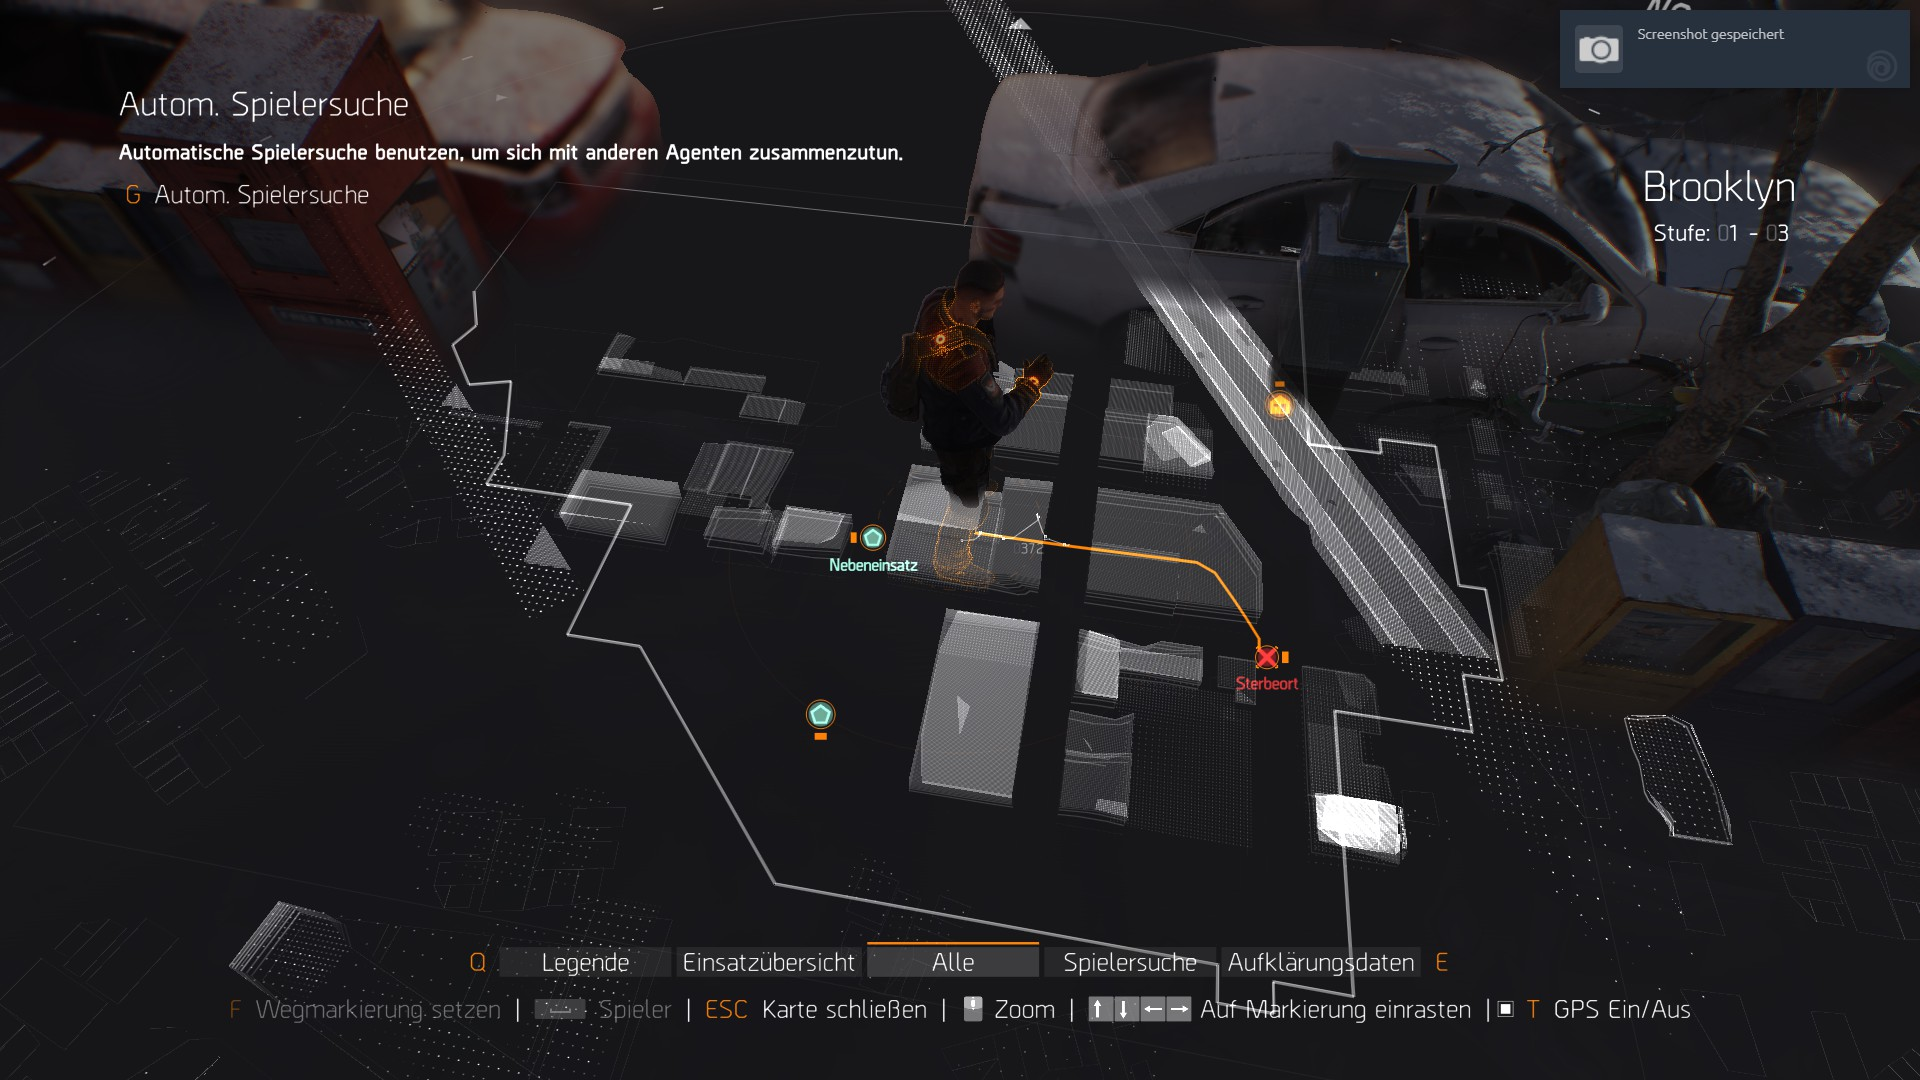
\includegraphics[width=\linewidth]{figures/concept/the_division_overlap}

    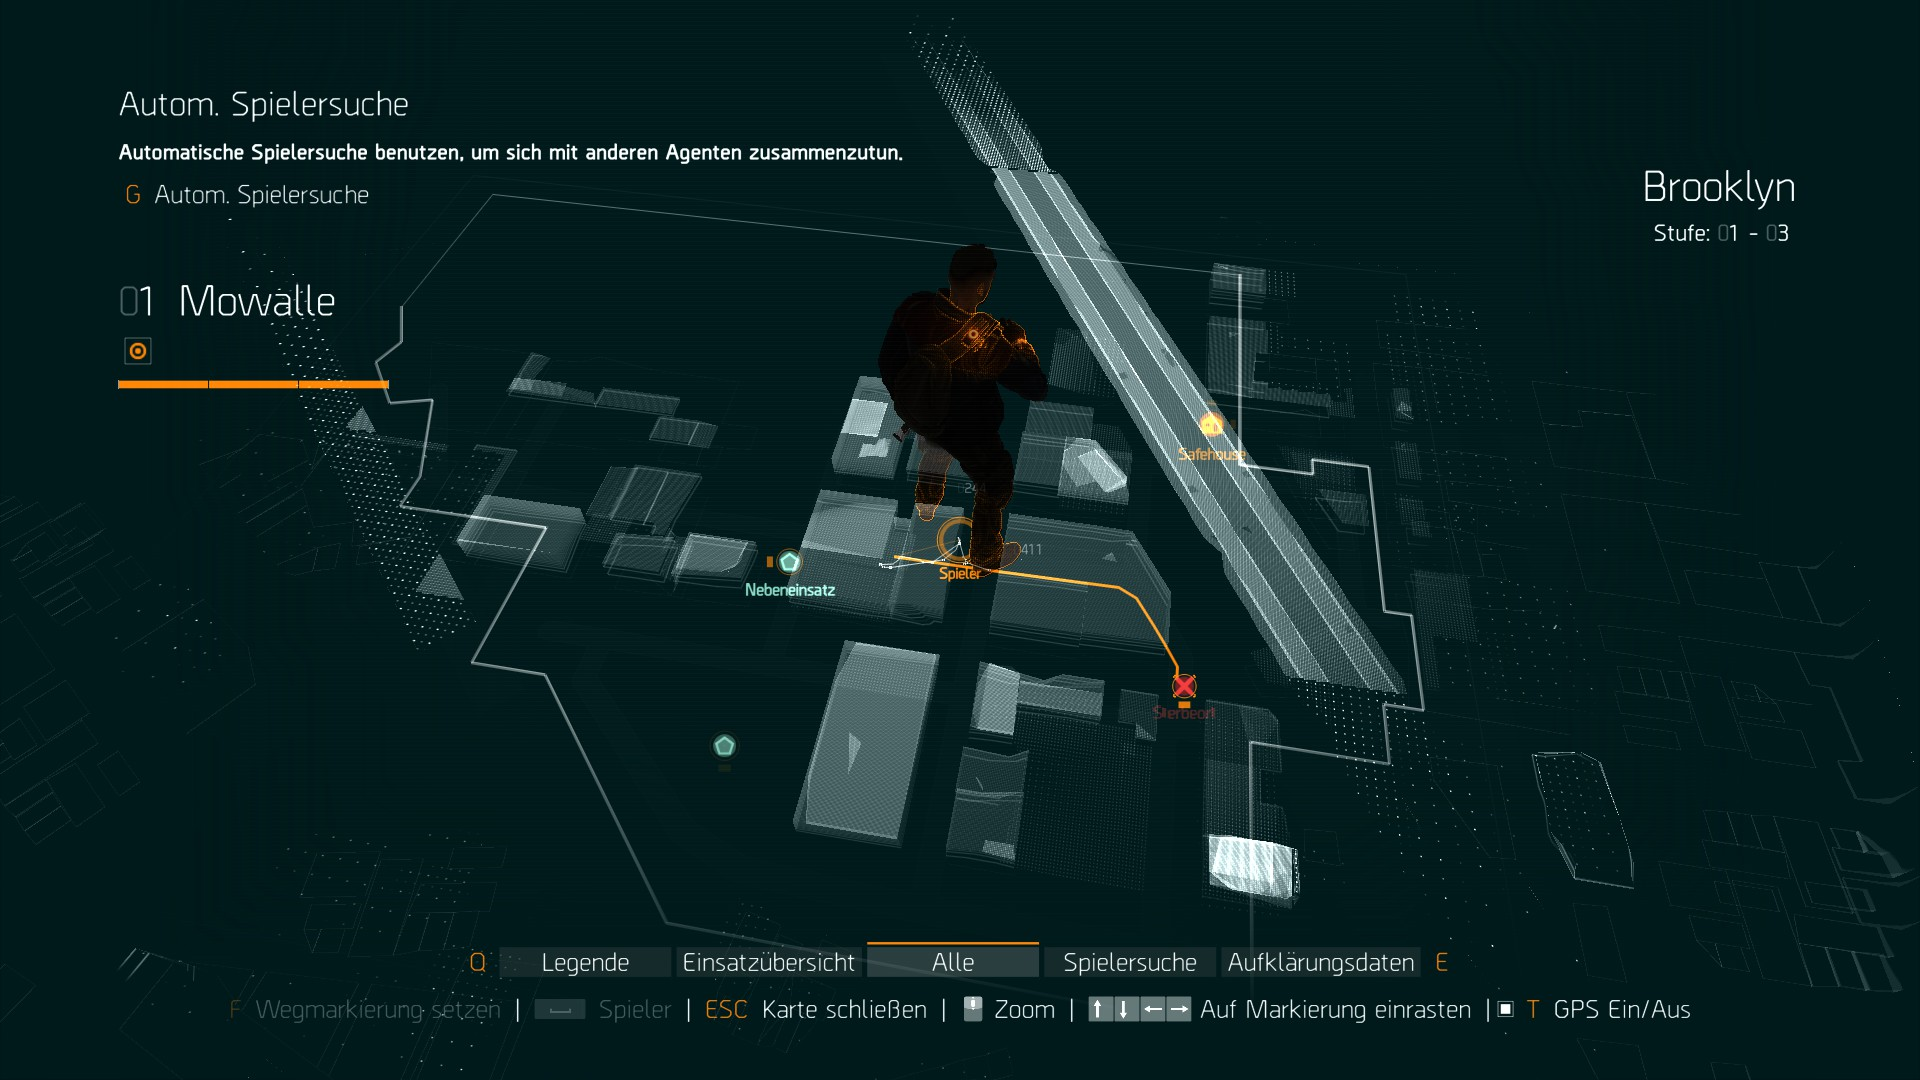
\includegraphics[width=\linewidth]{figures/concept/the_division_5}
    
    \caption{Übersicht der Magamap in TCTD.}
    \label{fig:tctd_overview}
\end{figure}

\begin{figure}[tbh]
    \centering
    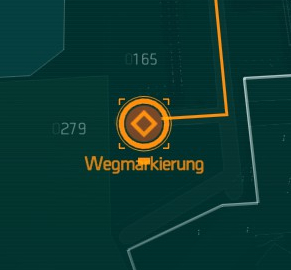
\includegraphics[width=0.3\linewidth]{figures/concept/the_division_clickmarker_x}
    \caption{Klickmarkierung in TCTDs Megamap mit x-/y-Koordinaten.}
    \label{fig:tctd_clickmarker}
\end{figure}

Die Megamap nutzt einige der Lokalisierungselemente, die auch in der anderen Anwendungen zu finden sind.
Ein Positionsmarker zeigt die aktuelle Position des Spielcharakters in der Welt an, wenn die Kamera nahe an die Karte herangezoomt wird.
Andernfalls bleibt der Spielcharakter sichtbar.
Straßen, Parks, Stadtteile etc. werden durch Text-Labels benannt.
Wichtige Punkte auf der Karte (wie zum Beispiel andere Spieler, Missionen, Gebäude oder Items) werden durch unterscheidbare Icons und ergänzenden Text markiert.
So können Spieler Orte auf der Karte schneller entdecken.
Mit dem Controller können die Spieler einen Cursor über die Megamap bewegen, der dabei x- und y-Koordinaten der Karte anzeigt.
Die Spieler können auch einen Klickmarkierung auf der Karte platzieren, welche automatisch eine Route vom Spielcharakter zum angeklickten Ort berechnet.
\autoref{fig:tctd_clickmarker} zeigt einen Screenshot der Klickmarkierung.

Falls stattdessen eine Ortsmarkierung angeklickt wird, werden die Attribute des Orts auf einem HUD angezeigt (siehe \autoref{fig:tctd_attributes}).
Beispielsweise werden bei einer Mission das notwendige Charakterlevel, die Missionsbeschreibung sowie die Belohnungen für einen Missionsabschluss aufgelistet.
Zudem werden die Entfernungen der Orte zum Spielcharakter angezeigt.
Diese Anzeige auf dem HUD ist vergleichbar mit den Attributslisten der anderen Kartenanwendungen.

Nähe-Elemente, wie es sie in den anderen Anwendungen gibt, sind in TCTD weniger zu finden.
Neben den positions- und zoomabhängigen Ortsmarkierungen und Entfernungsangaben bietet die Megamap in TCTD nur eine limitierte Funktionalität zum Filtern der Ortsmarkierungen.
Das Sortieren der Orte nach Kriterien, Umgebungsbilder oder eine offene Suche sind in der Megamap nicht vorhanden.
Öffnungszeiten oder Verkehrsinformationen gibt es in dem Spiel nicht.
Stattdessen werden die Positionen von anderen Mitspielern, Gegnern und Missionszielen in Echtzeit als Event-Elemente auf der Megamap präsentiert.

Da es sich bei der Megamap aus der Sicht des Spielcharakters um eine AR-Karte handelt, setzt sie einige Funktionen um, die mit den anderen Anwendungen nicht möglich sind.
Durch ihre Platzierung im 3D-Raum kann sie die Umrisse der Gebäude des virtuellen New Yorks auch in der Höhe darstellen.
Um die Megamap herum wird ein augmentierter Kompass-Ring eingeblendet, der den Spielern die Himmelsrichtungen anzeigt (teilweise sichtbar in \autoref{fig:tctd_attributes}).
Außerdem ist die Megamap mit einer augmentierten \enquote{GPS}-Routenführung für den Spielcharakter integriert.
Dabei zieht sich eine Linie durch die virtuelle Umgebung, welche den Spielern den Weg zu ausgewählten Zielen zeigt.
Einen Beispielscreenshot vom AR-GPS in TCTD findet sich in \autoref{fig:tctd_ar-gps}.

\begin{figure}[p]
    \centering
    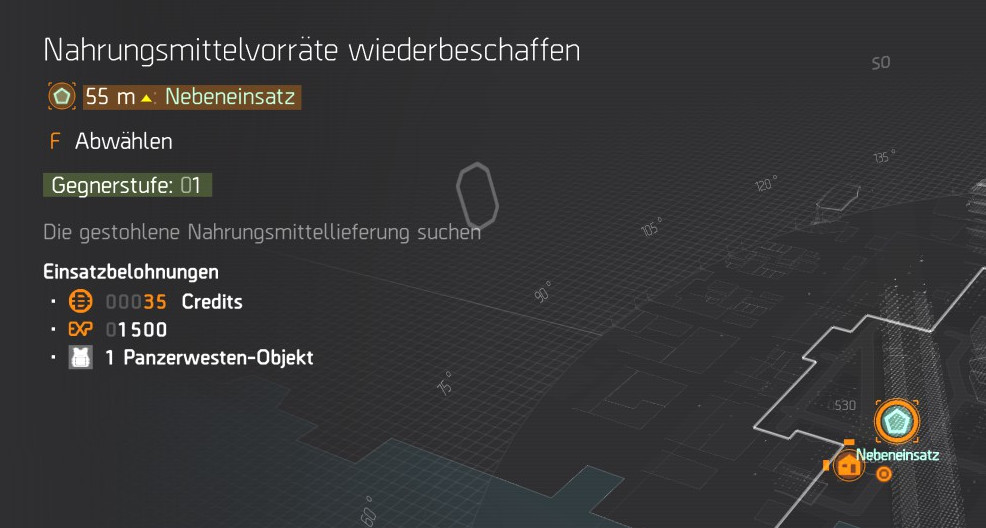
\includegraphics[width=\linewidth]{figures/concept/the_division_attributes_x}
    \caption{Durch Anklicken einer Ortsmarkierung werden die jeweiligen Daten zum Ort im HUD angezeigt.}
    \label{fig:tctd_attributes}
\end{figure}
\begin{figure}[p]
    \begin{minipage}{0.5\linewidth}
        \centering
        \vspace{0pt}
        \raisebox{-0.5\height}{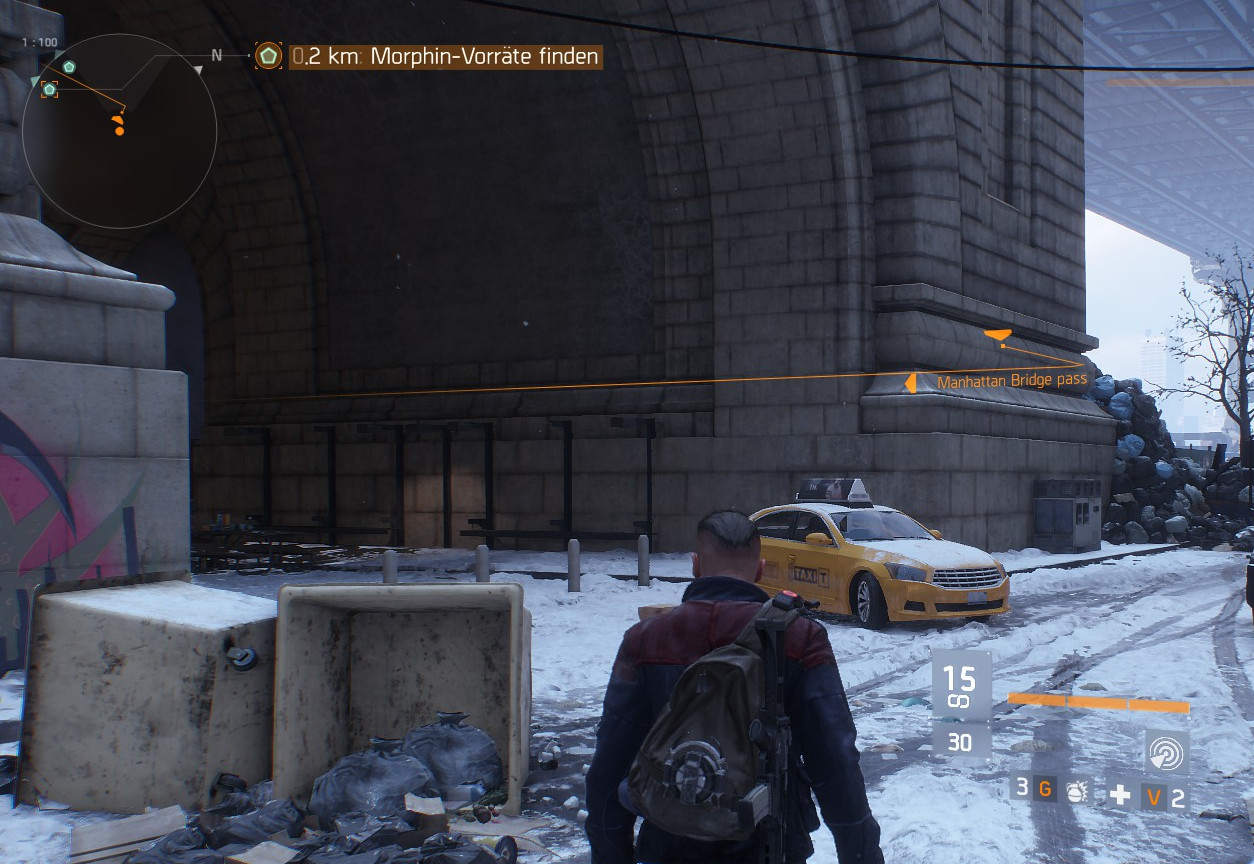
\includegraphics[width=\linewidth]{figures/concept/the_division_gps_x}}
    \end{minipage}%
    \hfill
    \begin{minipage}{0.48\linewidth}
        \centering
        \vspace{0pt}
        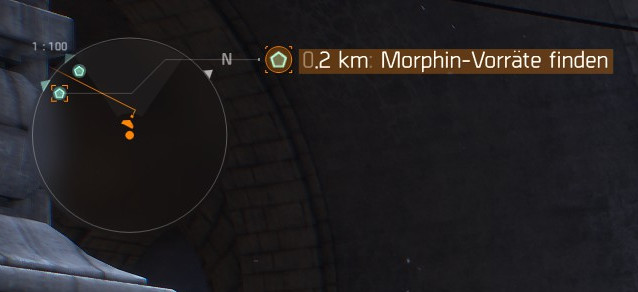
\includegraphics[trim={0, 3mm, 0, 2mm}, clip, width=\linewidth]{figures/concept/the_division_minimap}
        
        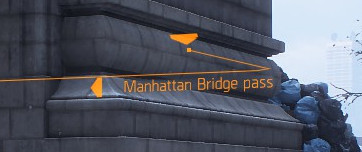
\includegraphics[trim={0, 1.5mm, 0, 1mm}, clip, width=\linewidth]{figures/concept/the_division_arrow}
    \end{minipage}
    \caption{Wegpunkt in Megamap kontrolliert das augmentierte GPS. %
    Oben~Rechts: Minikarte. %
    Unten~Rechts: Das GPS führt in Richtung \enquote{Manhattan Bridge pass}.}
    \label{fig:tctd_ar-gps}
\end{figure}

Viele Aspekte der Megamap in TCTD sind für die Umsetzung einer AR-Kartenanwendung in der realen Welt interessant.
Für die Realisierung einer solchen Anwendung ergeben sich allerdings Probleme, die gelöst werden müssen.
Zum Beispiel ist ein 3D-Modell der Umgebung in TCTD implizit gegeben, da die Umgebung selbst aus 3D-Modellen aufgebaut ist.
In der realen Welt sind Umgebungsmodelle selten verfügbar.
Damit eine Megamap dargestellt werden kann muss die Geometrie der Umgebung bekannt sein.
Dies ist auch für die Platzierung der Karte relevant.
Da im Spiel alle Umgebungsobjekte wie auch die Karte virtuell sind, können Überlappungen der Karte mit den Objekten durch visuelle Effekte wie in TCTD umgangen werden.
In der realen Welt muss die Megamap-Anwendung physische Objekte wahrnehmen können, um Überlappungen korrekt zu berechnen.
Ein weiteres Problem ist der Perspektivwechsel zwischen Erster- und Dritter-Person-Perspektive.
Die Megamap in TCTD ist nicht für den Spiel\emph{charakter}, sondern für den \emph{Spieler} selbst gedacht.
Das heißt, der Spieler betrachtet sowohl die virtuelle Umgebung als auch die Karte aus einer Dritte-Person-Perspektive.
In der realen Welt nehmen die Nutzer die Erste-Person-Perspektive ein, wodurch die Sicht auf die Megamap eine andere ist, als die im Spiel.
Es ist also nicht klar, ob sich das Konzept der Megamap auf die Anwendung in der Ersten-Person-Perspektive in der echten Welt übertragen lässt.

Auf diese Probleme wird im weiteren Verlauf der Arbeit durch die Aufstellung eines Megamap-Konzepts, dessen prototypischer Implementierung sowie einer Nutzerstudie des Prototyps eingegangen.

\section{Das Megamap-Konzept}
Basierend auf den Erkenntnissen der vorigen Abschnitte kann ein Konzept für eine umgebungsintegrierte Indoor-Megamap entwickelt werden, deren Zielplattform Mixed-Reality-HMDs sind.
Obwohl die untersuchten Kartenanwendungen für Außenbereiche ausgelegt sind, betrifft das in dieser Arbeit entwickelte Konzept Innenbereiche (Gebäude).
Wie \autoref{sec:motivation_ziel} bereits erwähnt ist der Grund hierfür, dass aktuelle MR-HMDs wie die HoloLens oder die Magic Leap in Außenbereichen kaum nutzbar sind.
Einerseits können sie die 3D-Strukturen der Umgebung nicht korrekt rekonstruieren.
Andererseits sind die virtuellen Inhalte auf den lichtdurchlässigen Brillen kaum erkennbar \parencite{Schroeder2017, Strange2018}.
Da das Konzept für Außenbereiche auf diesen HMDs nicht umsetzbar ist, wird die Megamap stattdessen für Innenbereiche entwickelt.
Das Konzept lässt sich dann zu einem späteren Zeitpunkt auf die Anwendung in Außenbereichen übertragen, sobald MR-HMDs die Nutzung im Freien unterstützen.

\subsection{Nutzungsszenario}
Die Megamap ist als eine dreidimensionale Karte für MR-HMDs konzipiert.
Vor dem Hintergrund der Umgebung des Nutzers zeigt sie ein dreidimensionales Innenmodell des Gebäudes, in dem sich der Nutzer zur Zeit befindet.
Die Karte wird durch das HMD in die Umgebung des Nutzers integriert.
Vor allem bleibt ihre Rotation in der Umgebung verankert, wenn der Nutzer sich bewegt.
Somit erscheint es, als würde die 3D-Karte tatsächlich ein Teil der Umgebung sein.
Für mehrstöckige Gebäude wird nur das aktuelle Stockwerk angezeigt, wobei Nutzer die Möglichkeit zum Wechsel der Stockwerke haben.
Über Interaktionselemente ist es möglich, Informationen zu Räumen und Objekten auf der Karte abzurufen.
Die Konzeptzeichnung in \autoref{fig:concept_overview} verdeutlicht das Prinzip.

Die Megamap soll Nutzern helfen, sich in unbekannten Gebäuden zu orientieren, diese zu erkunden und nach Orten in den Gebäuden zu suchen.
Ein Beispiel ist die augmentierte Exploration der Gebäude der Universität Bremen.
Neue Studierende oder Gäste der Universität können durch die Megamap bei der Suche nach Büros von Mitarbeitern, öffentlichen Druckern, Essensmöglichkeiten, Toiletten etc. unterstützt werden.
Da die meisten der Universitätsgebäude mehrstöckig sind, ist der Einsatz einer dreidimensionalen Karte zur Exploration interessant.
Auch der Einsatz in Einkaufszentren oder Flughäfen ist denkbar.
\begin{figure}[bht]
	\centering
    \framebox[\width]{
		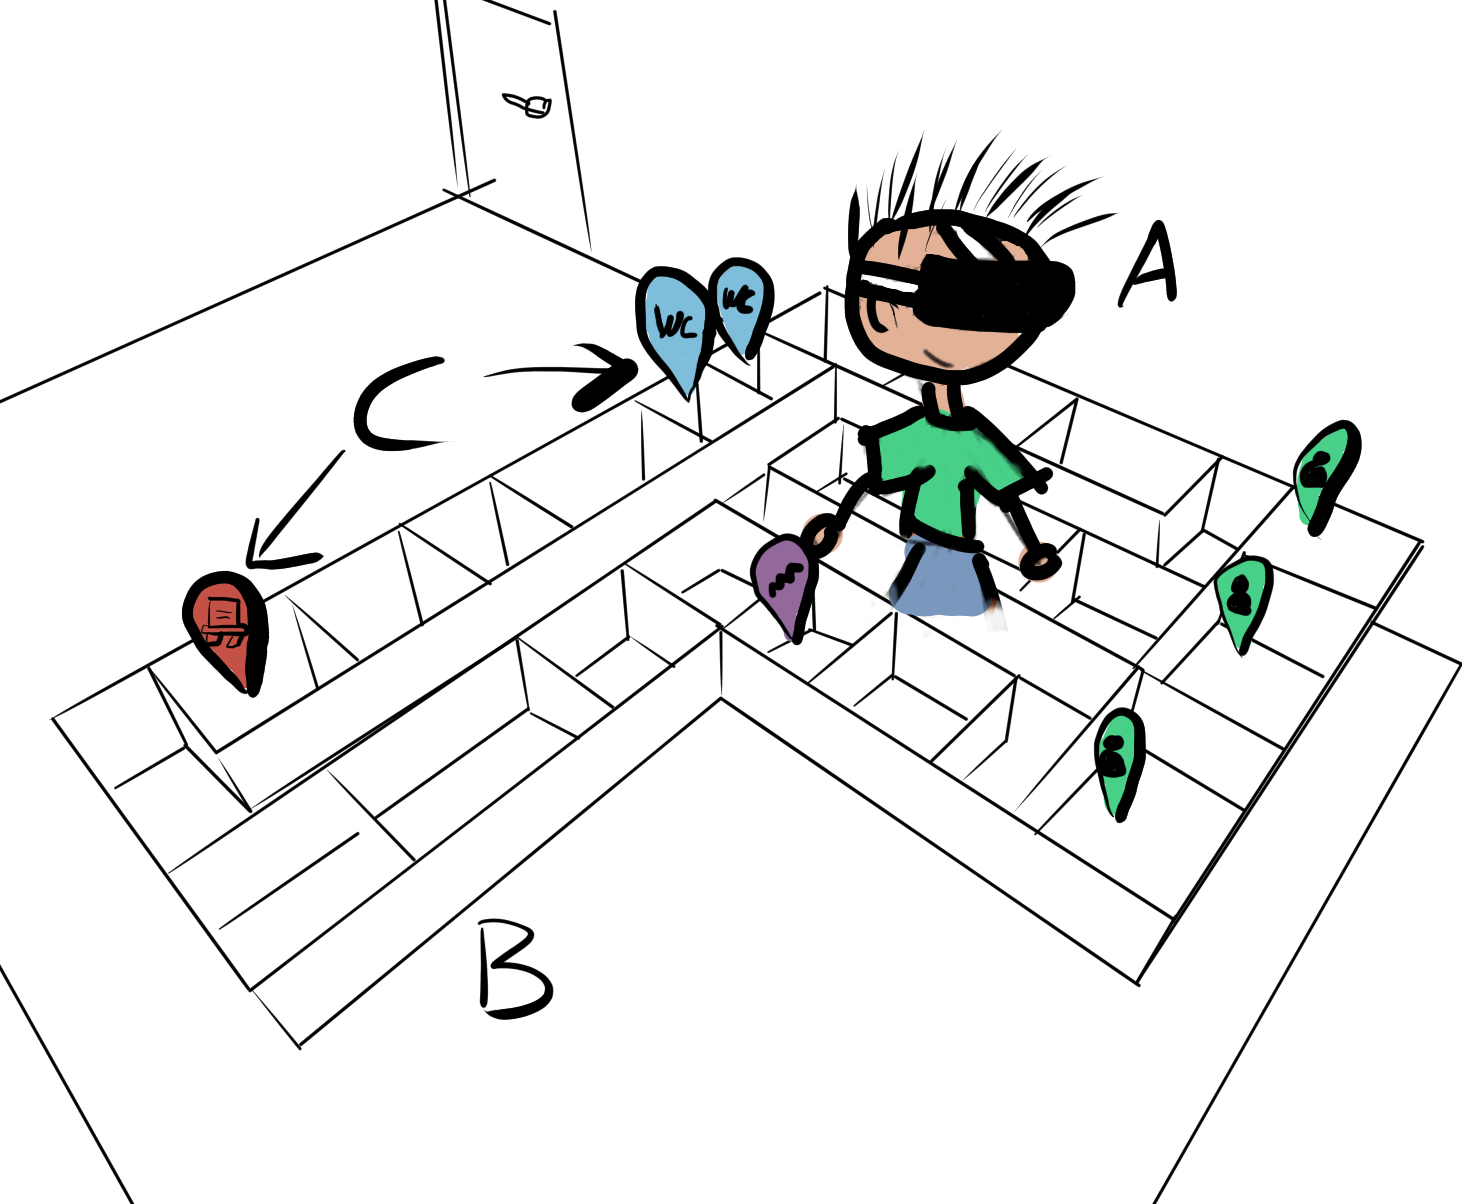
\includegraphics[width=0.75\linewidth]{figures/concept/overview}
	}
	\caption{Konzeptzeichnung einer Megamap. %
		A:~Nutzer trägt ein HMD. %
		B:~Indoor-Megamap wird in Umgebung des Nutzers angezeigt. %
		C:~Stecknadel-Icons markieren Räume mit Kategorien.}
	\label{fig:concept_overview}
\end{figure}

\subsection{Interaktion durch Explorationselemente}
Nutzern von MR-HMDs wie der HoloLens oder der Magic~Leap stehen drei Eingabemethoden zur Verfügung: Controller, Gesten- und Sprachsteuerung.
Da die Megamap in dieser Arbeit als Prototyp in VR implementiert wird, konzentriert sich das Konzept auf die Controller-Methode.

Damit das 3D-Gebäudemodell überhaupt als Karte fungieren kann, die müssen Nutzer mit dem Modell interagieren können.
Speziell muss die Karte Explorationselemente anbieten, mit denen die Nutzer die Umgebung erkunden können.
Mögliche Explorationselemente sind in \autoref{sec:exploration_elements} beschrieben.
Für das entwickelte Konzept sowie den Prototyp wurde eine kleine Auswahl der Elemente betrachtet.
In Zukunft sollte das Megamap-Konzept um weitere Explorationselemente ergänzt werden.

Für die Indoor-Megamap werden die Ortsmarkierungen als \emph{Raum}markierungen umfunktioniert.
Die Raummarkierungen werden als dreidimensionale Stecknadeln über Räumen mit besonderen Funktionen dargestellt.
So können interessante Orte im Gebäude hervorgehoben werden.
Durch Icons auf den Stecknadeln wird die Kategorie des Raums hervorgehoben (beispielsweise Büro, Toilette etc.).
Ebenso werden mit den Stecknadeln wichtige Objekte im Gebäude markiert (Drucker, Treppen und Aufzüge, Erste-Hilfe-Kästen etc.).
Über Filterelemente neben der Karte lassen sich Stecknadeln nach einer gewünschten Kategorie herausfiltern.
Die Konzeptzeichnung in \autoref{fig:concept_indoor_view} zeigt die Indoor-Megamap der Ebene 5 des MZH an der Universität Bremen.
Über eine virtuelle Filterbox werden nur Stecknadeln für öffentliche Toiletten gezeigt.
Stecknadeln werden auch über Stockwerke hinweg angedeutet, indem sie vertikal versetzt und transparent gemacht werden.
So können die Nutzer auch Orte und Objekte finden, die auf dem aktuellen Stockwerk nicht vorhanden sind.
\vfill
\begin{figure}[h]
	\centering
    \framebox[\width]{
		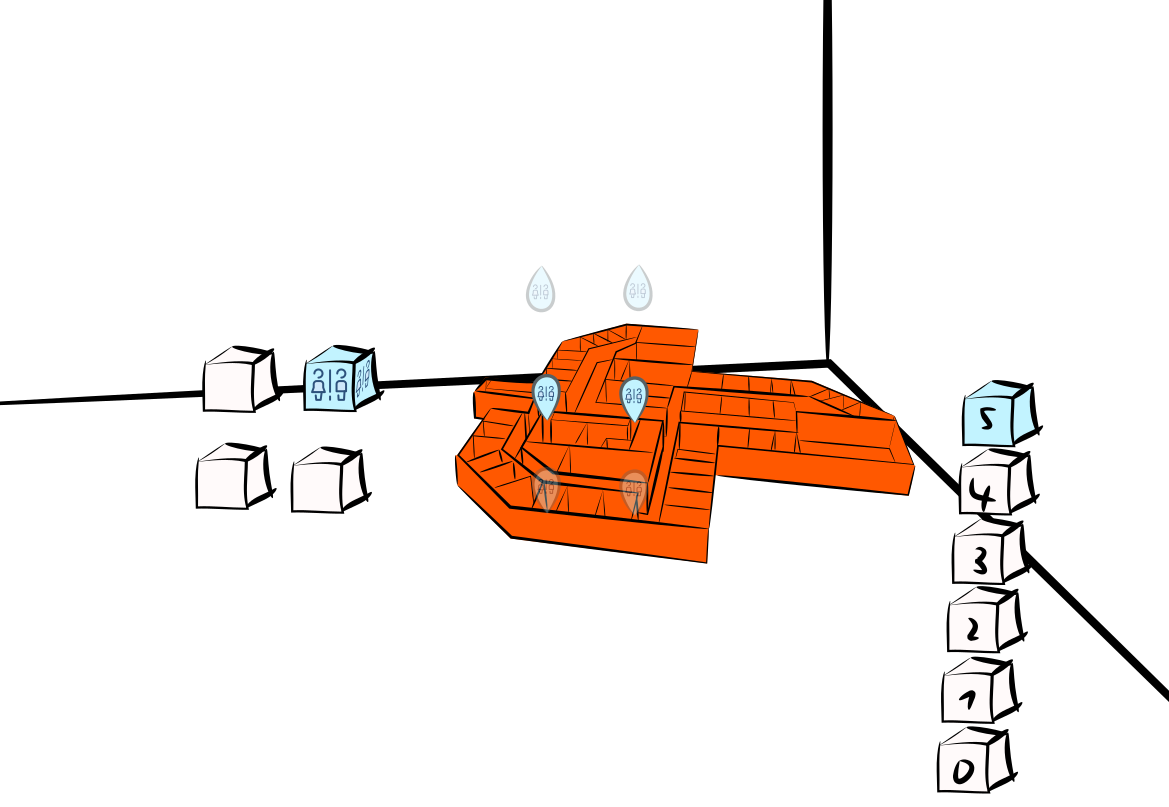
\includegraphics[trim={4cm, 0, 3cm, 5cm}, clip, width=0.7\linewidth]{figures/concept/3d_condition}
	}
	\caption{Konzeptzeichnung Megamap für Stockwerkwechsel, Filter und Suche.}
	\label{fig:concept_indoor_view}
\end{figure}

Um mehr Informationen zu einem Ort oder Objekt zu erhalten, können die Stecknadeln entweder mit dem im Raum getrackten Controller berührt werden, oder sie werden mit einem virtuellen Laserpointer anvisiert.
Letztere Variante hat den Vorteil, dass sich die Nutzer nicht zu weiter entfernten Stecknadeln hinbewegen müssen.
An der Position der Stecknadel öffnet sich ein Fenster mit Informationen zum Ort bzw. Objekt, was die Aufgabe der Attributsliste aus \autoref{sec:exploration_elements} abdeckt.
Ein Beispiel für ein solches Informationsfenster ist in \autoref{fig:concept_pin_info} skizziert.
Wie die Karte und die Stecknadeln ist auch das Informationsfenster in der Umgebung verankert.
Anstatt es direkt auf dem HMD als HUD anzuzeigen befindet sich das Fenster an der Position der Stecknadel und wird so rotiert, dass Nutzer immer auf die Vorderseite schauen.
Die relative Position des Fensters zur Umgebung bleibt gleich.
Eine Integration von 2D-Elementen als 3D-Objekt in die Umgebung (anstatt Anzeige als HUD) verhindert Unwohlsein bei den Nutzern sowie eine Verdeckung der Umgebung und anderer virtueller Inhalte \parencite{Schroeder2017}.
\begin{figure}[thb]
    \centering
        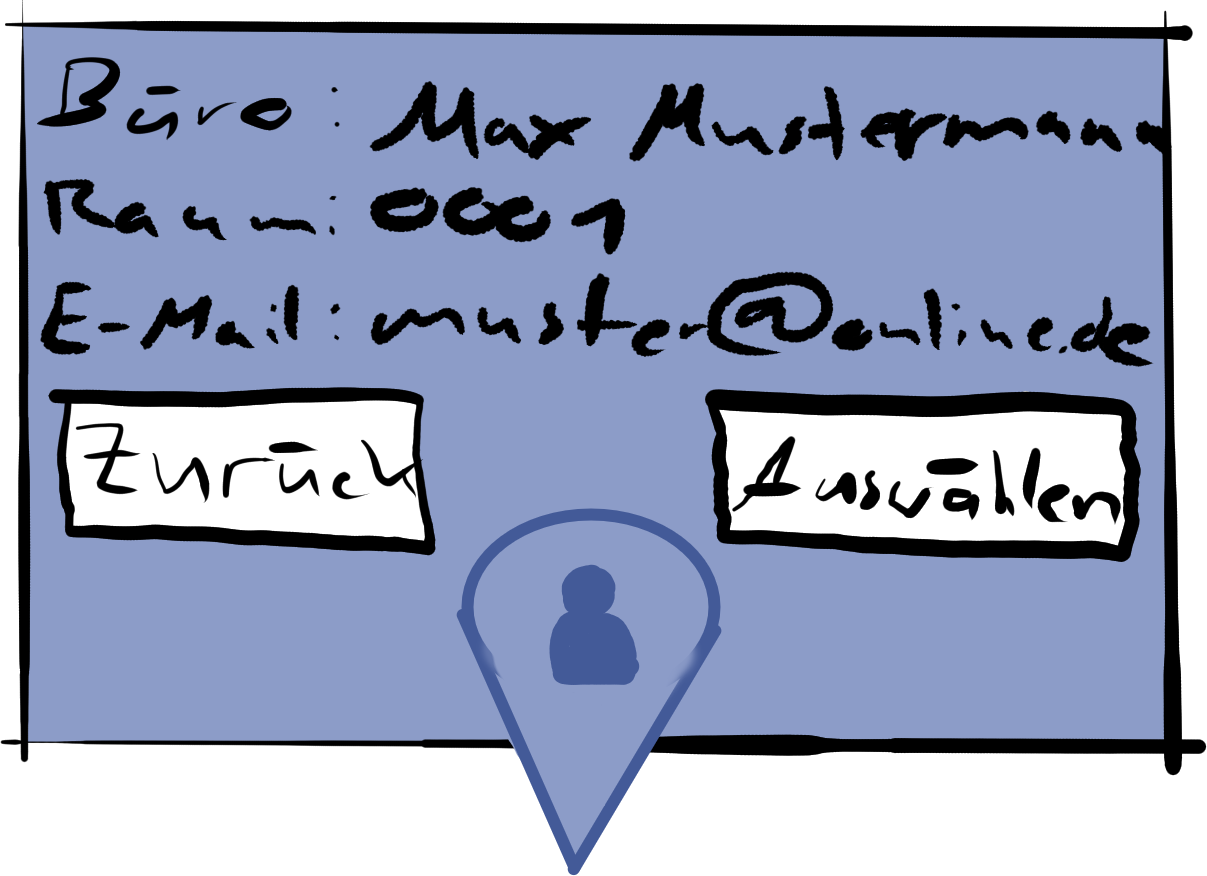
\includegraphics[width=0.5\linewidth]{figures/concept/concept_location_info}
    \caption{Konzeptzeichnung der Stecknadel-Informationen.}
    \label{fig:concept_pin_info}
\end{figure}

Zum Wechsel des aktuell gezeigten Stockwerks stehen weitere virtuelle Schaltflächen zur Verfügung (siehe \autoref{fig:concept_indoor_view}).
Mit diesen kann auf die gleiche Weise wie mit den Stecknadeln oder den Filterelementen über den Controller interagiert werden.
Die Nutzer müssen sich nicht tatsächlich auf das Stockwerk begeben, um es einsehen zu können.

Damit die Nutzer ihre Position auf der Karte schnell erkennen können wird der Positionsmarker als Lokalisierungselement für die Megamap übernommen.
Der Marker wird so platziert, dass er sich in der Megamap auf der Position der Nutzer befindet.
Für die 3D-Karte wird der Marker von einem zweidimensionalen Kreis zu einem Zylinder erweitert.
Zusätzlich zeigt ein Kegel die aktuelle Blickrichtung sowie den Blickwinkel der Nutzer an.

\subsection{Platzierung der Megamap im Raum}
Um die Megamap wie ein \enquote{reales} Objekt im Raum zu platzieren wird die 3D-Rekonstruktion des HMDs eingesetzt.
Durch die Rekonstruktion liefert das HMD 3D-Meshes des Bodens, der Wände und vereinfachte Meshes von Objekten in der Umgebung.
Die Megamap wird auf dem Mesh des Bodens platziert.
Überlagert in die reale Umgebung sieht es so aus, also stünde die Karte im Raum.

Analog zur Karte aus TCTD wird die Megamap bei der Aktivierung auf die Nutzer zentriert.
Das bedeutet, dass beim Aufrufen der Karte die Nutzer auf ihren eigenen Positionsmarkierungen stehen.
Dies soll den Nutzern eine schnellere Orientierung ermöglichen, da sie ihre Position auf der Karte nicht erst wiederfinden müssen.
Damit die Position der Nutzer bestimmt werden kann ist ein System zur Indoor-Lokalisierung erforderlich.
Mehrere Ansätze werden in der Literatur diskutiert, darunter \wifi-Fingerprinting \parencite{Lautenschlaeger2012, Alnabhan2014}, Magnetfeld-Fingerprinting \parencite{Hashish2017, Ang2018} oder Bild-basierte Verfahren \parencite{Kalkusch2002, Moeller2014, Silva2015}.
Weiterhin könnten die vom HMD gelieferten 3D-Meshes mit vorgefertigten Raummodellen abgeglichen werden, um den aktuellen Raum sowie die aktuelle Position der Nutzer zu bestimmen.

Ein Problem, das bei der Platzierung der virtuellen Karte in die reale Umgebung auftritt, ist die Verdeckung realer Objekte.
Sie dürfen, abhängig von ihrer Tiefe im Raum, nicht von der gerenderten Megamap verdeckt werden.
Andernfalls würde dies zu einem Bruch der Immersion sowie einer falschen Tiefenwahrnehmung der MR-Szene führen \cite{Kasperi2017, Walton2017}.
TCTD löst das Problem über die Transparenz der Megamap.
Die Karte wird effektiv an den Umgebungsobjekten \enquote{ausgeschnitten}.
Mit den erwähnten MR-HMDs ist ein solcher Effekt ebenfalls möglich.
Durch die 3D-Rekonstruktion ergeben sich grobe Meshes der Umgebungsobjekte und Wände.
Die virtuelle Megamap kann an den Stellen dieser Meshes transparent gerendert werden, wodurch der Effekt aus TCTD nachgestellt wird.

\subsection{Beschaffung von Gebäudedaten und Generierung der Karten}
Für die Darstellung als Megamap ist ein 3D-Modell des Gebäudes erforderlich.
Eine automatisierte Generierung des Modells basierend auf Gebäudedaten ist wünschenswert, damit das Modell nicht per Hand erstellt werden muss.
Ein möglicher Ansatz ist, die Grundrisse des jeweiligen Gebäudes zu georeferenzieren und in einer entsprechenden Datenbank wie z.\,B. OpenStreetMap zu veröffentlichen.
Die Megamap-Anwendung kann auf die georeferenzierten Grundriss-Daten über die Programmierschnittstelle (\emph{Application Programming Interface}, API) zugreifen und daraus 3D-Modelle generieren.
Die Wände des Gebäudes können z.\,B. als Polygon-Features mit dem OSM-Tag \lstinline{height} angelegt werden, die Türen würden durch Rechtecke mit dem Tag \lstinline{min_height} repräsentiert.
Normalerweise werden in OSM mit diesen Tags Gebäude als Ganzes definiert \parencite{OpenStreetMapFoundation2018b}.
Dennoch lassen sich die Tags für die Definition eines Indoor-Layouts umfunktionieren.

Ergänzend hierzu unterstützt OSM das \emph{Simple Indoor Tagging Schema}.
\autoref{fig:osm_simple-indoor-tagging} zeigt, wie das Schema auf ein Gebäudelayout angewendet werden kann.
Da dieses Schema zum regulären Tagging in OSM kompatibel ist, können Indoor- und Outdoor-Daten in der selben Datenbank verwaltet werden \parencite{OpenStreetMapFoundation2018c}.
Konkrete Möglichkeiten, die Daten aus OSM abzurufen und für die Megamap zu verwenden, werden in \autoref{chap:closing} diskutiert.
\begin{figure}[tbh]
    \centering
    \framebox[\width] {
        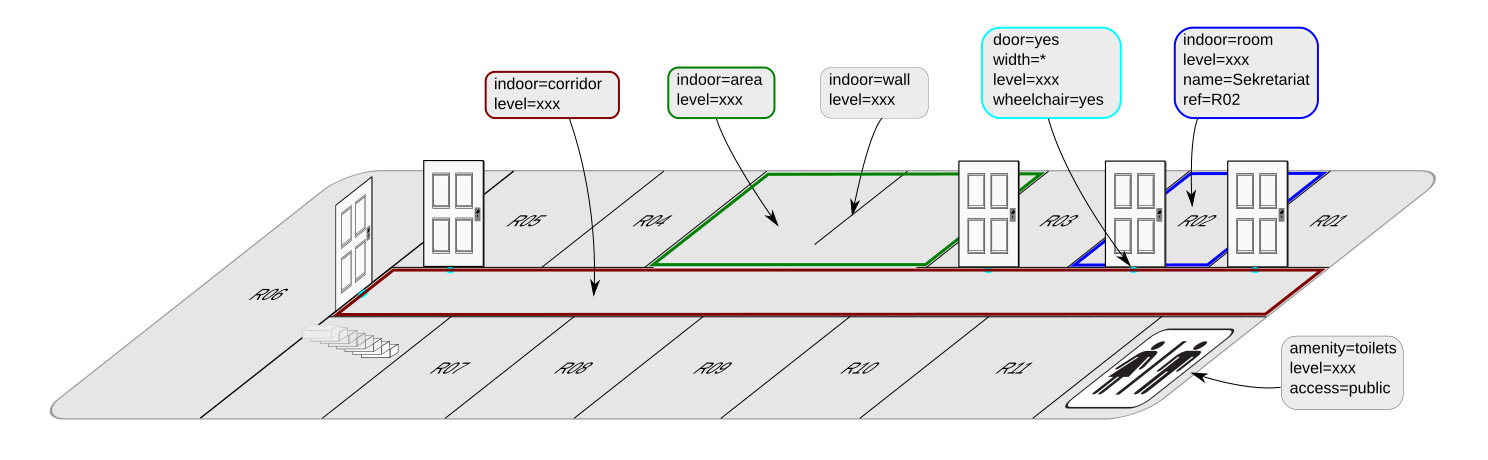
\includegraphics[trim={17cm, 0, 0, 0}, clip, width=0.9\linewidth]{figures/concept/osm_Indoor2_0_elements}
    }
    \caption{Beispiel des Simple Indoor Tagging Schemas in OpenStreetMap. %
    \quelle{\cite{OpenStreetMapFoundation2018c}; Ausschnitt durch Verfasser.}}
    \label{fig:osm_simple-indoor-tagging}
\end{figure}

%
\cleardoublepage
